\documentclass[8pt,twocolumn]{article}

\usepackage[
  paperwidth=180mm,
  paperheight=260mm,  
  left=20mm,right=20mm,
  top=18mm,bottom=20mm,
  includeheadfoot
]{geometry}
\setlength{\columnsep}{2mm}      

\usepackage[utf8]{inputenc}
\usepackage[T2A]{fontenc}
\usepackage[russian]{babel}
\usepackage{microtype}

\usepackage{tempora}   
\usepackage{newtxmath}
\usepackage{amsmath,amssymb}

\usepackage{graphicx}
\usepackage[table]{xcolor}
\usepackage{array}
\usepackage{booktabs}
\usepackage{caption}

\newcolumntype{C}[1]{>{\centering\arraybackslash}p{#1}}

\setlength{\parskip}{4pt}
\setlength{\parindent}{1.25em}

\usepackage{fancyhdr}
\pagestyle{fancy}
\fancyhf{}

\newcommand{\MyHeader}{
  \parbox{\textwidth}{\centering
    \thepage\\[-2pt]
    \rule{\textwidth}{0.4pt}\\[-1pt]
    {\normalsize {\MakeUppercase{Что такое функция?}}}
  }
}

\renewcommand{\headrulewidth}{0pt}
\fancyhead[C]{\MyHeader}
\setlength{\headheight}{32pt}

\usepackage[normalem]{ulem}

\usepackage{tabularx}
\newcolumntype{Y}{>{\centering\arraybackslash}X}

\usepackage[norule]{footmisc}


\begin{document}

В школьных учебниках пишут, что «числовая плоскость» — это такая плоскость, на которой некоторым определённым образом введены координаты. Если верить учебникам буквально, то числовых плоскостей очень много. Проводя на классной доске оси координат, учитель превращает в «числовую плоскость» плоскость этой доски; ученики на страницах своих тетрадок изготавливают всё новые и новые «числовые плоскости», иногда по нескольку на одной странице!

В школьном курсе алгебры чаще всего имеют дело с функциями, заданными «аналитически», то есть при помощи формулы. Область определения такой функции, если не сказано ничего другого, считается множеством всех тех значений аргумента, для которых все предписанные формулой операции над числами выполнимы. Будем, например, как это принято в школе, считать знак $\sqrt{\phantom{x}}$ знаком «арифметического» квадратного корня. Ясно, что формула
\begin{equation}\tag{9}
y=f(x)=(\sqrt{x})^2
\end{equation}
позволяет вычислить по заданному $x$ соответствующее ему значение $y$ лишь при неотрицательном $x$ (иначе квадратный корень «не извлекается»).

При неотрицательном $x$
\begin{equation}\tag{10}
y=f(x)=x.
\end{equation}
Формула (10) проще, чем формула (9), и хотелось бы её считать формулой, определяющей нашу функцию. Но область определения функции, заданной формулой (10), состоит не из одних неотрицательных чисел $x$, а из всех чисел $x$. Если мы хотим дать новое определение той самой функции, которая была определена формулой (9), надо написать
\begin{equation}\tag{11}
y=f(x)=
\left\{
\begin{array}{l@{}l} 
  x, & \text{при } x\ge 0,\\
  \text{не определена}, & \text{при } x<0.
\end{array}
\right.
\end{equation}

Подобным же образом функцию
\[
g(x)=\dfrac{x^3-1}{x-1}
\]
можно записать так:

\vspace{-1.6\baselineskip}
\begin{equation}\tag{12}
g(x)=
\begin{cases}
x^2+x+1, & \text{при } x\ne 1,\\
\text{не определена}, & \text{при } x=1.
\end{cases}
\end{equation}
\vspace{-1.2\baselineskip}

На школьных и вузовских экзаменах требуют полной точности в подобных вопросах.

\vspace{-0.6\baselineskip}
\section*{\centering \normalsize График функции}
\vspace{-1.0\baselineskip}

Рассмотрим следующий график дежурств.

\begin{figure}[h]
\centering
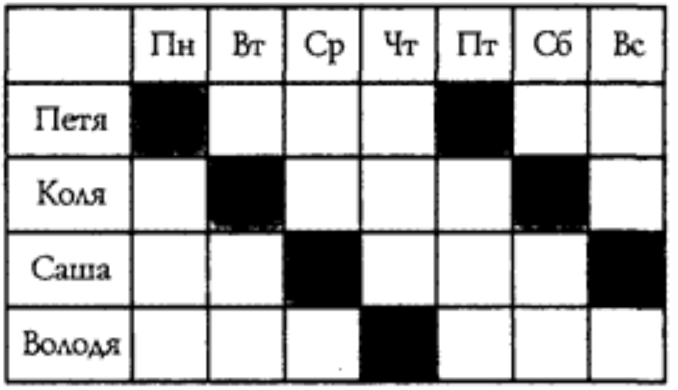
\includegraphics[width=\linewidth,height=40mm]{schedule1.png}
\end{figure}
\vspace{-0.2\baselineskip}

Мы уже знаем, что это график функции: имя дежурного можно считать значением функции от аргумента «день недели». Так как дней недели семь, а мальчиков четверо, то мы нарисовали

\vspace{-1.0\baselineskip}
\[
7\times4=28
\]
клеточек, но отметили только семь из них. Если бы мальчики решили расположить свои имена по алфавиту, то получилась бы следующая табличка:

\begin{figure}[h]
\centering
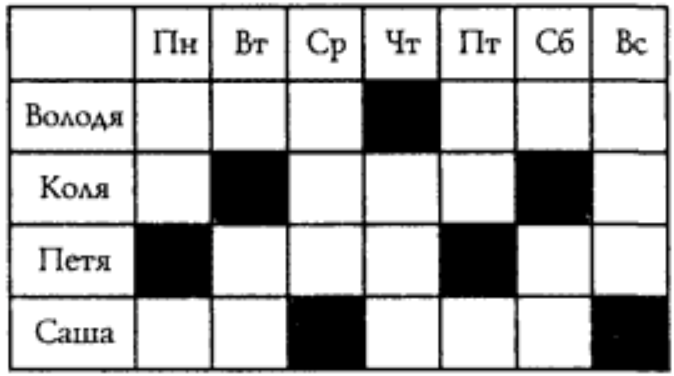
\includegraphics[width=\linewidth,height=40mm]{schedule2.png}
\end{figure}
\vspace{-0.2\baselineskip}

Выглядит она по-другому, но изображает то же самое распределение дежурств - ту же самую функцию.

В обеих таблицах 28 клеточек соответствуют 28 возможным парам. 

\begin{center}
\emph{(день недели, мальчик)}
\end{center}

Из этих 28 пар выделены семь пар. 

(пн, Петя), (вт, Коля), (ср, Саша), (чт, Володя), (пт, Петя), (сб, Коля), (вс, Саша), т.е. все пары, в которых день недели соединен с дежурным на этот день:

\emph{(день недели, дежурный на этот день)}, или абстрактно: пары вида

\vspace{-1.0\baselineskip}
\[
(x, f(x)).
\]
\vspace{-1.4\baselineskip}

Только выбор этих пар и существенен для задания функции. 

После этого примера вам, быть может, не покажется неожиданным такое определение: \emph{графиком функции $f$ называется множество всех таких пар\footnote{\emph{Всюду в этой статье имеются в виду «упорядоченные пары». Пара (1,2) отличается от пары (2,1). Первый и второй элементы пары могут и совпадать: (1,1) или (2,2) - тоже пары.}}}
\[
(x,y),
\]
\emph{что: 1) первый элемент пары $x$ принадлежит области определения функции, 2) второй элемент пары $y=f(x)$.}

В нашем примере график функции $f$:

Г$_{f}$=\{(пн, Петя), (вт, Коля), (ср, Саша), (чт, Володя), (пт, Петя), (сб, Коля), (вс, Саша)\},

Для фукнций, заданных таблицей

\vspace{-0.6\baselineskip}
\begin{center}
\setlength{\tabcolsep}{6pt}
\renewcommand{\arraystretch}{1.15}
\begin{tabularx}{\linewidth}{|Y|Y|Y|Y|Y|}
\hline
$x$ & $f_1$ & $f_2$ & $f_3$ & $f_4$ \\ \hline
$A$ & $A$   & $B$   & $A$   & $B$   \\ \hline
$B$ & $A$   & $B$   & $B$   & $A$   \\ \hline
\end{tabularx}
\end{center}
\vspace{-0.4\baselineskip}
в соответствии с данным определением получим графики
\[
\begin{aligned}
\text{Г}_{1}&=\{(A,A),(B,A)\}, & \text{Г}_{2}&=\{(A,B),(B,B)\},\\
\text{Г}_{3}&=\{(A,A),(B,B)\}, & \text{Г}_{4}&=\{(A,B),(B,A)\}.
\end{aligned}
\]


Ясно, что для функций с конечной областью определения число элементов графика (т.е. число входящммх в график пар) равно числу элементов области определения функции. Для функций с бесконечной областью определения все пары
\end{document}
